\documentclass[a4paper, 12pt]{article}
\usepackage{amsmath}
\usepackage{pgfplots}
\usetikzlibrary{datavisualization}
\usepackage{float}
\usetikzlibrary{hobby}
\usepackage{graphicx}
\usepackage{twemojis}
\usepackage{caption}
\usepackage{subcaption}
\usepackage{mdframed}   
\usepackage{framed}
\newmdenv[]{kotak}
\begin{document}
\textbf{Solutions to}
\bigbreak
Exam: Calculus II, 22 June 2022 
\bigbreak
\textbf{done by Sonia} (I just decided to learn LaTeX this way, okay??)\\
\bigbreak
\bigbreak
\textbf{Ex. 1.} Let \(f(x) = x^3\) on [0, \emph{a}], \emph{a} $>$ 0.
\bigbreak
(a) Calculate lower and upper Riemann sums for corresponding to the partition of [0, \emph{a}] into \emph{n} equal subintervals.
\bigbreak
(b) What is the difference between upper and lower Riemann sums?
\bigbreak
Hint. Use the formula \[ \sum_{k=1}^{n} k^3 = \frac{n^2(n+1)^2}{4}. \]
\bigbreak
\textbf{Solution:}
\[ \emph{U(f, P)} =  \sum_{k=1}^{n} f(u_k) \Delta x_k. \]
\[ \emph{L(f, P)} =  \sum_{k=1}^{n} f(l_k) \Delta x_k. \]
\[ P_n: 0 < \frac{a}{n} < ... < \frac{na}{n} = a \]
\begin{align*}
x_k = \frac{ka}{n} \,\,\,\,\,\,\,\,\,\,\,\,\,\,\,\, x_{k-1} = \frac{(k-1)a}{n}\\\\
\Delta x_k = \frac{ka}{n} - \frac{(k-1)a}{n} = \frac{a}{n}
\end{align*}
\bigbreak
(a) Riemann sums:
\begin{align*}
\emph{U(f, P)} = \sum_{k=1}^{n} [\frac{ka}{n}]^3 \,\, \frac{a}{n} \,\, 
= \sum_{k=1}^{n} \frac{k^3 a^3}{n^3} \,\, \frac{a}{n} \,\, 
= \sum_{k=1}^{n} k^3 \,\, \frac{a^4}{n^4} \,\, 
= \frac{a^4}{n^4} \,\, \sum_{k=1}^{n} k^3 \,\, 
= \frac{a^4}{n^4} \,\, \frac{n^2(n+1)^2}{4}\\\\
= \frac{a^4}{4} \,\, \frac{(n+1)^2}{n^2}.
\end{align*}
\begin{align*}
\emph{L(f, P)} = \sum_{k=1}^{n} [\frac{(k-1)a}{n}]^3 \,\, \frac{a}{n} \,\, 
= \sum_{k=1}^{n} \frac{(k-1)^3 a^3}{n^3} \,\, \frac{a}{n} \,\, 
= \sum_{k=1}^{n} (k-1)^3 \,\, \frac{a^4}{n^4} \,\, 
= \frac{a^4}{n^4} \,\, \sum_{k=1}^{n} (k-1)^3 \\\\ 
= \frac{a^4}{n^4} \,\, \frac{(n-1)^2((n-1)+1)^2}{4} \,\,
= \frac{a^4}{n^4} \,\, \frac{(n-1)^2 n^2}{4} \,\,
= \frac{a^4}{4} \,\, \frac{(n-1)^2}{n^2}.
\end{align*}
\bigbreak
\bigbreak
(b) Difference:
\begin{align*}
\emph{U(f, P)} - \emph{L(f, P)} \,\, = \,\, \frac{a^4}{4} \,\, \frac{(n+1)^2}{n^2} \,\, - \,\, \frac{a^4}{4} \,\, \frac{(n-1)^2}{n^2} \,\, = \,\, \frac{a^4}{4} \,\, \frac{(n+1)^2 - (n-1)^2}{n^2}\\\\
= \,\, \frac{a^4}{4} \,\, \frac{n^2 + 2n + 1 - n^2 + 2n - 1}{n^2}
\,\, = \,\, \frac{a^4}{4} \,\, \frac{4n}{n^2}
\,\, = \,\, \frac{a^4}{4} \,\, \frac{4}{n}
\,\, = \,\, \frac{a^4}{n}.
\end{align*}
\textbf{P.S.:} Mr Maligranda mentioned that he wanted us to find this difference (b) in a different way, but it is \underline{not} specified in the task itself. But we can try to show limits:
\bigbreak
\begin{align*}
\lim_{n \to \infty} U(f, P) \,\, = \,\, \lim_{n \to \infty} \frac{a^4}{4} \,\, \frac{(n+1)^2}{n^2} \,\, = \,\, \frac{a^4}{4} \,\, \lim_{n \to \infty} \frac{n^2 + 2n + 1}{n^2} \\\\
= \,\, \frac{a^4}{4} \,\, \lim_{n \to \infty} \frac{1 + \frac{2}{n} + \frac{1}{n^2}}{1} 
\,\, = \,\, \frac{a^4}{4}.
\end{align*}
\bigbreak
\begin{align*}
\lim_{n \to \infty} L(f, P) \,\, = \,\, \lim_{n \to \infty} \frac{a^4}{4} \,\, \frac{(n-1)^2}{n^2} \,\, = \,\, \frac{a^4}{4} \,\, \lim_{n \to \infty} \frac{n^2 - 2n + 1}{n^2} \\\\
= \,\, \frac{a^4}{4} \,\, \lim_{n \to \infty} \frac{1 - \frac{2}{n} + \frac{1}{n^2}}{1}
\,\, = \,\, \frac{a^4}{4}.
\end{align*} \\\\
\textbf{Ex. 2.}
\bigbreak
(a) Find the function $F(x) = \int_{0}^x f(t)dt$ for $x \in [0,3]$ if
\bigbreak
\begin{equation*}
\emph{f(x)} =
	\begin{cases}
	x - 1 & \text{if } 0 \leq x \leq 1,\\
	-2x + 4 & \text{if } 1 < x \leq 2,\\
	1 & \text{if } 2 < x \leq 3.
	\end{cases}
\end{equation*}
(b) Draw the graphs of \emph{f} and \emph{F}. \\
(c) Find left-derivatives and right-derivatives at $x = 1$ and at $x = 2$, i.e.,

\begin{align*}
F'(1^-) = \lim_{h \to 0^-} \,\, \frac{F(1 + h) - F(1)}{h}, \,\, F'(2^-) = \lim_{h \to 0^-} \,\, \frac{F(2 + h) - F(2)}{h},
\end{align*}
and
\begin{align*}
F'(1^+) = \lim_{h \to 0^+} \,\, \frac{F(1 + h) - F(1)}{h}, \,\, F'(2^+) = \lim_{h \to 0^+} \,\, \frac{F(2 + h) - F(2)}{h}.
\end{align*}
Is \emph{F} differentiable at 1 and/or at 2?
\bigbreak
\textbf{Solution:}\\\\
(a)\\\\
\twemoji[scale=0.5]{1f438} \,\, $0 \leq x \leq 1$:
\begin{align*}
F(x) = \int_{0}^x (t - 1) \,\, dt \,\, = \,\, (\frac{1}{2} t^2 - t)\Bigr|_{0}^{x} \,\, = \,\, 
\frac{1}{2} x^2 - x.
\end{align*}
\twemoji[scale=0.5]{1f438} \,\, $1 < x \leq 2$:
\begin{align*}
F(x) = \int_{0}^1 (t - 1) \,\, dt + \int_{1}^x (-2t + 4) \,\, dt 
\,\, = \,\, (\frac{1}{2} t^2 - t)\Bigr|_{0}^{1} + (-t^2 + 4t)\Bigr|_{1}^{x} \,\, = \,\, 
-x^2 + 4x - \frac{7}{2}.
\end{align*}
\twemoji[scale=0.5]{1f438} \,\, $2 < x \leq 3$:
\begin{align*}
F(x) = \int_{0}^1 (t - 1) \,\, dt + \int_{1}^2 (-2t + 4) \,\, dt 
+ \int_{2}^x 1 \,\, dt
\,\, = \,\, (\frac{1}{2} t^2 - t)\Bigr|_{0}^{1} + (-t^2 + 4t)\Bigr|_{1}^{2} + t\Bigr|_{2}^{x}\\ = \,\, 
x - \frac{3}{2}.
\end{align*}
\newpage
(b)\\
\begin{figure}[H]
  \begin{subfigure}{0.4\textwidth}
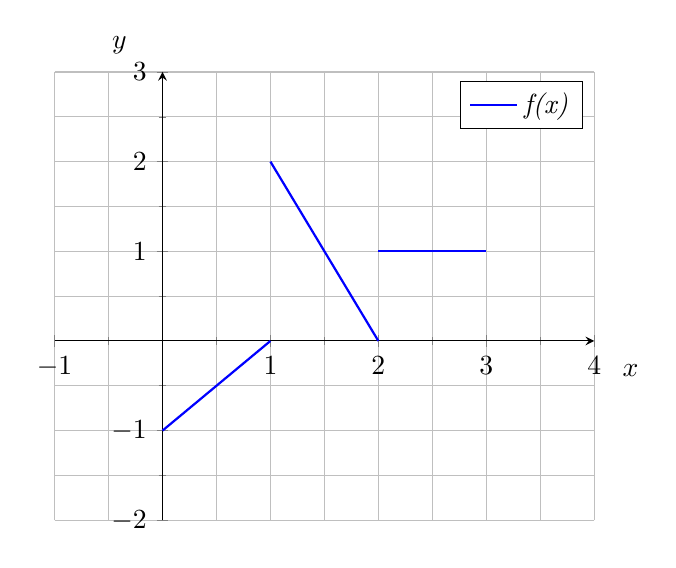
\begin{tikzpicture}
\begin{axis}[grid=both,ymin=-2,ymax=3,xmax=4,xmin=-1,
      minor tick num=1,axis lines = middle,xlabel=$x$,ylabel=$y$,label style =
      {at={(ticklabel cs:1.1)}}]
    \addplot [mark=none, thick, blue] coordinates {(0,-1) (1,0)};
    \addplot [mark=none, thick, blue] coordinates {(1,2) (2,0)};
    \addplot [mark=none, thick, blue] coordinates {(2,1) (3,1)};
    \legend{\emph{f(x)}}
\end{axis}
\end{tikzpicture}
  \end{subfigure}
  \hfill
  \begin{subfigure}{0.4\textwidth}
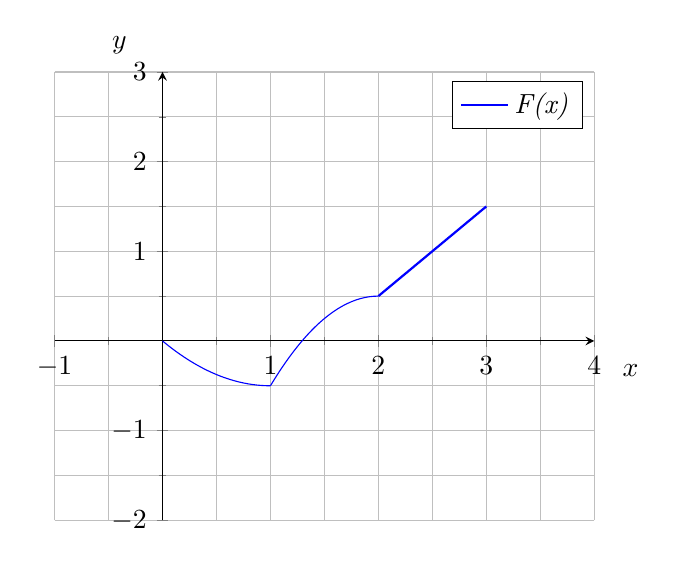
\begin{tikzpicture}
\begin{axis}[grid=both,ymin=-2,ymax=3,xmax=4,xmin=-1,
      minor tick num=1,axis lines = middle,xlabel=$x$,ylabel=$y$,label style =
      {at={(ticklabel cs:1.1)}}]
    \addplot [smooth, hobby, tension=5, domain = 0:1, blue] (\x, {0.5 * \x^2 - \x});
    \addplot [smooth, hobby, tension=5, domain = 1:2, blue] (\x, {-\x^2 + 4*\x - 7/2});
    \addplot [thick, blue] coordinates {(2,0.5) (3,1.5)};
    \legend{\emph{F(x)}}
\end{axis}
\end{tikzpicture}
  \end{subfigure}
\end{figure}
(c)\\
\begin{align*}
F'(1^-) \,\, = \,\, \lim_{h \to 0^-} \frac{F(1 + h) - F(1)}{h}
\,\, = \,\, \lim_{h \to 0^-} \frac{\frac{1}{2}(1 + h)^2 - (1 + h) + \frac{1}{2}}{h} \\\\ 
= \,\, \lim_{h \to 0^-} \frac{\frac{1}{2} + h + \frac{1}{2}h^2 - 1 - h + \frac{1}{2}}{h}
\,\, = \,\, \lim_{h \to 0^-} \frac{\frac{1}{2}h^2}{h}
\,\, = \,\, \lim_{h \to 0^-} \frac{1}{2}h \,\, = \,\, 0.
\end{align*}\\
\begin{align*}
F'(1^+) \,\, = \,\, \lim_{h \to 0^+} \frac{F(1 + h) - F(1)}{h}
\,\, = \,\, \lim_{h \to 0^+} \frac{-(1 + h)^2 + 4(1 + h) - \frac{7}{2} + \frac{1}{2}}{h} \\\\
= \,\, \lim_{h \to 0^+} \frac{-1 - 2h - h^2 + 4 + 4h - 3}{h}
\,\, = \,\, \lim_{h \to 0^+} \frac{-h^2 + 2h}{h} 
\,\, = \,\, \lim_{h \to 0^+} (-h + 2) \,\, = \,\, 2.
\end{align*}\\
Since $0 = F'(1^-) \not = F'(1^+) = 2$, \emph{F} is \underline{not} differentiable at 1.
\bigbreak
\begin{align*}
F'(2^-) \,\, = \,\, \lim_{h \to 0^-} \frac{F(2 + h) - F(2)}{h}
\,\, = \,\, \lim_{h \to 0^-} \frac{-(2 + h)^2 + 4(2 + h) - \frac{7}{2} - \frac{1}{2}}{•} \\\\
= \,\, \lim_{h \to 0^-} \frac{-4 - 4h - h^2 + 8 + 4h - 4}{h}
\,\, = \,\, \lim_{h \to 0^-} (-h) \,\, = \,\, 0.
\end{align*}
\begin{align*}
F'(2^+) \,\, = \,\, \lim_{h \to 0^+} \frac{F(2 + h) - F(2)}{h}
\,\, = \,\, \lim_{h \to 0^+} \frac{2 + h - \frac{3}{2} - \frac{1}{2}}{h} \\\\
\,\, = \,\, \lim_{h \to 0^+} 1 \,\, = \,\, 1.
\end{align*}\\
Since $0 = F'(2^-) \not = F'(2^+) = 1$, \emph{F} is \underline{not} differentiable at 2.
\bigbreak
\bigbreak
\textbf{Ex. 3.} (a) Find the partial sums
\begin{align*}
G_n = \sum_{k=3}^{n} (\frac{2}{3})^k \, , \,\,\, T_n = \sum_{k=3}^{n} \frac{1}{k(k+2)} \,\,\,\, \text{for} \,\,\,\, n \geq 3.
\end{align*} 
\begin{equation*}
\text{(b) Find sum of the series} \,\, \sum_{k=3}^{\infty} \left[(\frac{2}{3})^k + \frac{1}{k(k+2)}\right].
\end{equation*}
\bigbreak
\textbf{Solution:}
\bigbreak
\centerline{\textbf{Preamble}}
\begin{framed}
The formula used for Geometric n-series:
\begin{equation*}
\sum_{i=m}^{n} r^i \,\, = \,\, \frac{r^m - r^{n+1}}{1-r}.
\end{equation*}       
\end{framed}
\bigbreak
\bigbreak
(a)\\\\
\twemoji[scale=0.5]{1f438} \,\, $G_n:$\\
\begin{align*}
S_n = \frac{\left(\frac{2}{3}\right)^3 - \left(\frac{2}{3}\right)^{n+1}}{1 - \frac{2}{3}}
\,\, = \,\, \frac{\frac{8}{27} - \frac{2^{n+1}}{3^{n+1}}}{\frac{1}{3}}
\,\, = \,\, \frac{8}{9} - \frac{2^{n+1}}{3^n}.
\end{align*}
\newpage
\twemoji[scale=0.5]{1f438} \,\, $T_n:$\\
\begin{gather*}
S_n = \sum_{k=3}^{n} \frac{1}{k(k+2)} = \frac{1}{2} \,\, \sum_{k=3}^{n} \frac{1}{k} - \frac{1}{k+2} = \frac{1}{2} \,\, [ \frac{1}{3} - \frac{1}{5} + \frac{1}{4} - \frac{1}{6} + ... +
\frac{1}{n-4} - \frac{1}{n-2} \\\\ + \frac{1}{n-3} - \frac{1}{n-1} + \frac{1}{n-2} - \frac{1}{n} +  \frac{1}{n-1} - \frac{1}{n+1} + \frac{1}{n} - \frac{1}{n+2} ]
 = | cancelling \,\, out | \\\\ =  \frac{1}{2} \,\, [ \frac{1}{3} + \frac{1}{4} - \frac{1}{n+1} - \frac{1}{n+2}] = \frac{7}{24} + \frac{-2n - 3}{2(n+2)(n+1)} = 
\frac{7(n+2)(n+1) - 12(2n+3)}{24(n+2)(n+1)} \\\\ = \frac{7n^2 + 21n + 14 - 24n - 36}{24(n+2)(n+1)} = \frac{7n^2 - 3n - 22}{24(n + 2)(n+1)}.
\end{gather*}
\bigbreak
(b) \\\\
\begin{equation*}
\lim_{n \to \infty} \left[ \frac{8}{9} - \frac{2^{n+1}}{3^n} \right] = \frac{8}{9}.
\end{equation*}
\bigbreak
\begin{equation*}
\lim_{n \to \infty} \left[ \frac{7n^2 - 3n - 22}{24(n + 2)(n+1)} \right]
= \lim_{n \to \infty} \left[ \frac{7n^2 - 3n - 22}{24(n^2 + 3n + 2)} \right] 
= \frac{1}{24} \,\, \lim_{n \to \infty} \frac{7 - \frac{3}{n} - \frac{22}{n^2}}{1 + 
\frac{3}{n} + \frac{2}{n^2}} = \frac{7}{24}.
\end{equation*}
\bigbreak
Since both of the series converge:
\begin{align*}
\sum_{k=3}^{\infty} \left[(\frac{2}{3})^k + \frac{1}{k(k+2)}\right] = 
\sum_{k=3}^{\infty} (\frac{2}{3})^k + \sum_{k=3}^{\infty} \frac{1}{k(k+2)} = 
\frac{8}{9} + \frac{7}{24} = \frac{85}{72}.
\end{align*}
\newpage
\textbf{Ex. 4.} Find global maximum and global minimum of the function \\
\[ f(x, y) = x^2 y^2 + x^3 y - 4x^2 y \]
over triangle with vertices (0, 0), (0, 6), (6, 0).
\bigbreak
\textbf{Solution:}
\begin{gather*}
f_x = xy(3x + 2y - 8)\\
f_y = x^2(x + 2y - 4)\\\\
\begin{cases}
xy(3x + 2y - 8) = 0;\\
x^2(x+2y - 4) = 0;
\end{cases}\\\\
\begin{cases}
3(4 - 2y) + 2y - 8= 0;\\
x = 4 - 2y;
\end{cases}\\\\
\begin{cases}
12 - 4y -8=0;\\
x = 4-2y;
\end{cases}\\\\
\begin{cases}
y = 1;\\
x = 2.
\end{cases}
\end{gather*}
Which gives us \underline{\emph{P(2, 1)}}.\\\\
\twemoji[scale=0.5]{1f438} \,\, (0, 0) and (0, 6):\\\\
$f(0, y) = 0.$\\\\
\twemoji[scale=0.5]{1f438} \,\, (0, 0) and (6, 0):\\\\
$f(x, 0) = 0.$\\\\
\newpage
\twemoji[scale=0.5]{1f438} \,\, (0, 6) and (6, 0):
\begin{gather*}
y = -x + 6\\\\
f(x, -x+6) = x^2(-x + 6)^2 + x^3(-x+6) -4x^2(-x+6)\\
= (6 -x)(6x^2 - x^3 +x^3 -4x^2) = 2x^2(6-x).\\\\
f' = (12x^2 - 2x^3)' = 24x - 6x^2.\\
24x - 6x^2 = 0\\
6x(4-x) = 0\\
x = 0 \,\,\, \text{or} \,\,\, x = 4
\end{gather*}
Therefore:
\begin{gather*}
\begin{cases}
y = -x+6;\\
x = 4;
\end{cases}\\\\
\begin{cases}
y = 2;\\
x = 4;
\end{cases}
\end{gather*}
Which gives us \underline{\emph{P(4, 2)}}.\\\\
Therefore, global extrema are:
\begin{gather*}
f(2, 1) = -4.\\
f(4, 2) = 64.
\end{gather*}
\newpage
\textbf{Ex. 5.} Solve the differential equation\\
\[ y'' -2y' = 6 \, e^{2x}. \]\\
(b) Solve the initial value problem\\
\begin{gather*}
\begin{cases}
y'' - 2y' = 6 \, e^{2x},\\
y(0) = 1,\\
y'(0) = 2.
\end{cases}
\end{gather*}
\bigbreak
\textbf{Solution:}\\
\begin{framed}
All solutions of differential equation:
\begin{equation*}
y = y_H + y_P.
\end{equation*}       
\end{framed}
(a) \\
\[ y'' -2y' = 6 \, e^{2x}. \]
1) \underline{homo}geneous:
\begin{gather*}
y'' - 2y' = 0\\
\lambda^2 - 2\lambda = 0\\
\lambda(\lambda - 2) = 0\\
\lambda_1 = 0 \,\,\, \text{or} \,\,\, \lambda_2 = 2\\\\
\text{Since } \lambda_1 \not = \lambda_2 \text{ real:}\\
\underline{y_H = C_1 e^{0x} + C_2 e^{2x} = C_1 + C_2 e^{2x}}.
\end{gather*}
2) particular:
\begin{gather*}
y_P = Axe^{2x}.\\
y_P' = Ae^{2x} + 2Axe^{2x} = Ae^{2x} (1 + 2x).\\
y_P'' = 2Ae^{2x}(1+2x) + 2Ae^{2x} = 2Ae^{2x}(2x + 2).\\\\
2Ae^{2x}(2x + 2) - 2Ae^{2x} (1 + 2x) = 6e^{2x}\\
2Ae^{2x}(2x + 2 - 1 - 2x) = 6e^{2x}\\
2A = 6\\
A = 3\\\\
\text{Therefore: } \underline{y_P = 3xe^{2x}}.\\\\
\text{Then, all solutions of the differential equation: }\\
\underline{y = C_1 + C_2 e^{2x} + 3xe^{2x}}.
\end{gather*}
\newpage
(b) \\
\begin{gather*}
y = C_1 + C_2 e^{2x} \,\,\,\,\,\,\, \textbf{from homogeneous part of point (a)}\\\\
\text{From the initially given conditions:}\\
\begin{cases}
y(0) = 1,\\
y'(0) = 2.
\end{cases}\\\\
y(0) = C_1 + C_2 e^0 = C_1 + C_2. \,\,\,\,\, \text{and} \,\,\,\,\, y(0) = 1\\\\
\text{Which gives us: } \underline{C_1 + C_2 = 1}.\\\\
y' = 2C_2e^{2x}\\
y'(0) = 2C_2 \,\,\,\,\, \text{and} \,\,\,\,\, y'(0) = 2\\\\
\text{Which gives us: } \underline{C_2 = 1}.\\\\
\text{Therefore: }\\
\begin{cases}
C_1 + C_2 = 1;\\
C_2 = 1;
\end{cases}\\
\begin{cases}
C_1 =0;\\
C_2 = 1;
\end{cases}
\end{gather*}\\\\
\textbf{Therefore, the solution to IVP:} \[\underline{y = e^{2x}}.\] 
\bigbreak
\bigbreak
\textbf{P.S.:} I am \underline{not} sure in the solution to IVP, but hopefully it is correct.\\\\\\
\begin{framed}
Good luck with retake preparation and may the odds be even in your favor!     
\end{framed}

\end{document}